\documentclass[10pt,twocolumn]{article}
\usepackage[spanish]{babel}
\usepackage{graphicx}
\usepackage{float}
\usepackage{microtype}

\title{Estudio de percolación 2D}
\author{Murillo barra Espitia Jaime, Rodríguez P. Nicolás, Torres Julián} 

\begin{document}
\maketitle

\section{Resumen}
    Se simuló el llenado aleatorio de una malla bidimensional de tamaño $L\times L$para estudiar la percolación de sitio. Para generar la malla se
    utilizó un vector de vectores, y sus elementos se ocuparon con una distribución aleatoria uniforme con rango entre 0.0 y 1.0.
    Un sitio de la matriz se ocupa si su número aleatorio correspondiente es menor o igual a la probabilidad de llenado $p$.
    Ya con sitios ocupados y vacíos, se procede a verificar si se forman clusters entre los sitios ocupados (teniendo en cuenta
    solo vecinos inmediatos), y a cada uno se le asigna una etiqueta o identificador. Si una etiqueta aparece en la primera y en la última fila
    y/o en la primera y en la última columna, significa que el cluster identificado con dicha etiqueta es percolante. El tamaño de cada cluster
    se calcula contando cuántos elementos existen por cada etiqueta. Finalmente, se reporta el tamaño promedio del cluster percolante más grande
    $s(p, L)$ y la probabilidad $P(p, L)$ de que exista un cluster percolante para distintos valores de $p$ y $L$.

\section{Introducción}
    La teoría de percolación es una rama fundamental de la física estadística que estudia el comportamiento de sistemas aleatorios 
    conectados, con aplicaciones que van desde la propagación de fluidos en medios porosos hasta la transmisión de enfermedades en redes 
    complejas \cite{stauffer1994introduction}. El concepto central de percolación se basa en determinar si existe un 
    camino conectado que atraviese completamente un sistema aleatorio, fenómeno conocido como transición de percolación.\\

    En sistemas bidimensionales, la percolación consiste en ocupar aleatoriamente los lugares de una red regular con probabilidad $p$, 
    donde cada sitio puede estar ocupado (1) o (0). Los sitios ocupados que son vecinos inmediatos (conectados en cruz) forman clusters 
    conectados. El sistema presenta percolación cuando existe al menos un cluster que conecta bordes opuestos de la red, ya sea horizontal 
    o verticalmente.\\

    Uno de los aspectos más importantes de la percolación es la existencia de un umbral crítico $p_c$, donde ocurre una transición de fase. 
    Para $p < p_c$, típicamente solo existen clusters finitos, mientras que para $p > p_c$ aparece un cluster infinito que abarca todo el 
    sistema. En redes cuadradas bidimensionales, el valor crítico teórico es $p_c = 0.5927...$.\\

    El estudio computacional de la percolación requiere algoritmos eficientes para identificar y caracterizar clusters conectados. El 
    algoritmo de Hoshen-Kopelman \cite{hoshen1976percolation} es particularmente útil para este propósito, ya que permite identificar 
    clusters en una sola pasada sobre la red utilizando técnicas de Union-Find optimizadas.\\

    En este trabajo, implementamos una simulación computacional de percolación de sitio en redes cuadradas bidimensionales de diferentes
    tamaños ($L \times L$), utilizando el algoritmo de Hoshen-Kopelman para identificar clusters conectados. Nuestro objetivo es calcular la 
    probabilidad de percolación $P(p,L)$ y caracterizar estadísticamente el tamaño de los clusters percolantes para diferentes valores de la 
    probabilidad de ocupación $p$ y tamaños de sistema $L$.\\

    
\section{El problema} 
    
\section{El código}
    Estas son las funciones principales usadas para el estudio:

    $fill\_matix(L, p, gen):$ Llena la matriz con una distribución uniforme de números entre 0.0 y 1.0. Luego, convierte
    dichos números en 1 si son menores o iguales a $p$. Si no, los convierte en 0.\\ 

    $Hoshen\_Kopelman(matrix, L):$ Recorre la matriz verificando si los sitios ocupados tienen vecinos, de ser así los agrupa
    y les asigna una etiqueta única.\\

    $check\_if\_pecolant(matrix, L):$ Verifica si hay etiquetas que aparezcan tanto en la primera fila como en la última, o
    en la primera columna como en la última. De ser así, arroja un 1 indicando que hay percolación y la etiqueta del cluster.\\
    
    $count(matrix, L, idx):$ Cuenta el número de elementos de la matriz que poseen la o las etiquetas mostradas por
    $check\_if\_pecolant(matrix, L)$.\\

    En el cálculo de las estadísticas se emplearon las funciones de $statistic.cpp$. Las funciones $print\_matrix(matrix, L)$
    y $print\_sizes(matrix, L)$ fueron usadas en etapas tempranas del código para verificar su funcionamiento. La primera 
    imprime las coordenadas de de cada sitio junto con su etiqueta, y la segunda imprime los tamaños de los clusters
    percolantes.\\ 

\section{Pruebas}
    Como primer acercamiento al problema, se usó las función $print\_matrix(matrix, L)$ para visualizar los espacios ocupados
    en la matriz. La figura \ref{64 0.5} muestra en amarillo los sitios ocupados con una probabilidad $p = 0.5$ de una matriz
    de tamaño $64\times 64$, mientras que la figura \ref{merged 64 0.5} muestra otra prueba con los sitios ocupados agrupados
    en clusters de diferentes colores. En este caso específico, no hay percolación. 
   \begin{figure}[H]
    \centering
    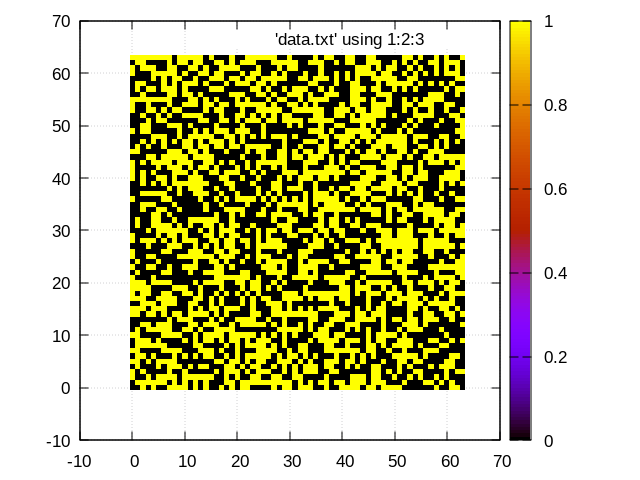
\includegraphics[width=9cm]{data/64 0.5.png}
    \caption{Matriz $64\times 64$ con $p = 0.5$.}
    \label{64 0.5} 
   \end{figure} 

   \begin{figure}[H]
    \centering
    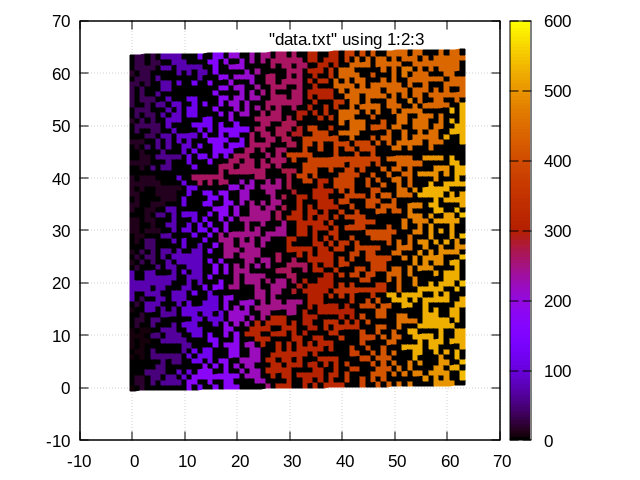
\includegraphics[width=9cm]{data/merged 64 0.5.png}
    \caption{Matriz $64\times 64$ con $p = 0.5$ con los sitios ocupados agrupados en clusters.}
    \label{merged 64 0.5} 
   \end{figure} 

\section{Resultados} 
   bubub
    
   \section{Referencias}
   \begin{thebibliography}{99}
   
   \bibitem{stauffer1994introduction}
   Stauffer, D., \& Aharony, A. (1994). \textit{Introduction to percolation theory}. CRC press.
   
   \bibitem{hoshen1976percolation}
   Hoshen, J., \& Kopelman, R. (1976). Percolation and cluster distribution. I. Cluster multiple labeling technique and critical 
   concentration algorithm. \textit{Physical Review B}, 14(8), 3438.
   
   \end{thebibliography}
   


\end{document}
